\subsubsection{Validación de computacional}

Para validar la estructura previamente definida se tomó en consideración los pesos de todos los sistemas que serán montados en esta estructura, así como el peso máximo generado por la materia orgánica que el sistema es capaz de procesar.

Para validar la estructura se hicieron 2 estudios, un estudio de esfuerzos, para ver los puntos críticos de la estructura que podrían sufrir alguna ruptura debido al peso aplicado, y otro de las deformaciones generadas por este mismo peso
 (Figura \ref{fg:Estructura1}) (Figura \ref{fg:Estructura2}). 
 
\begin{figure}[h]
    \centering
        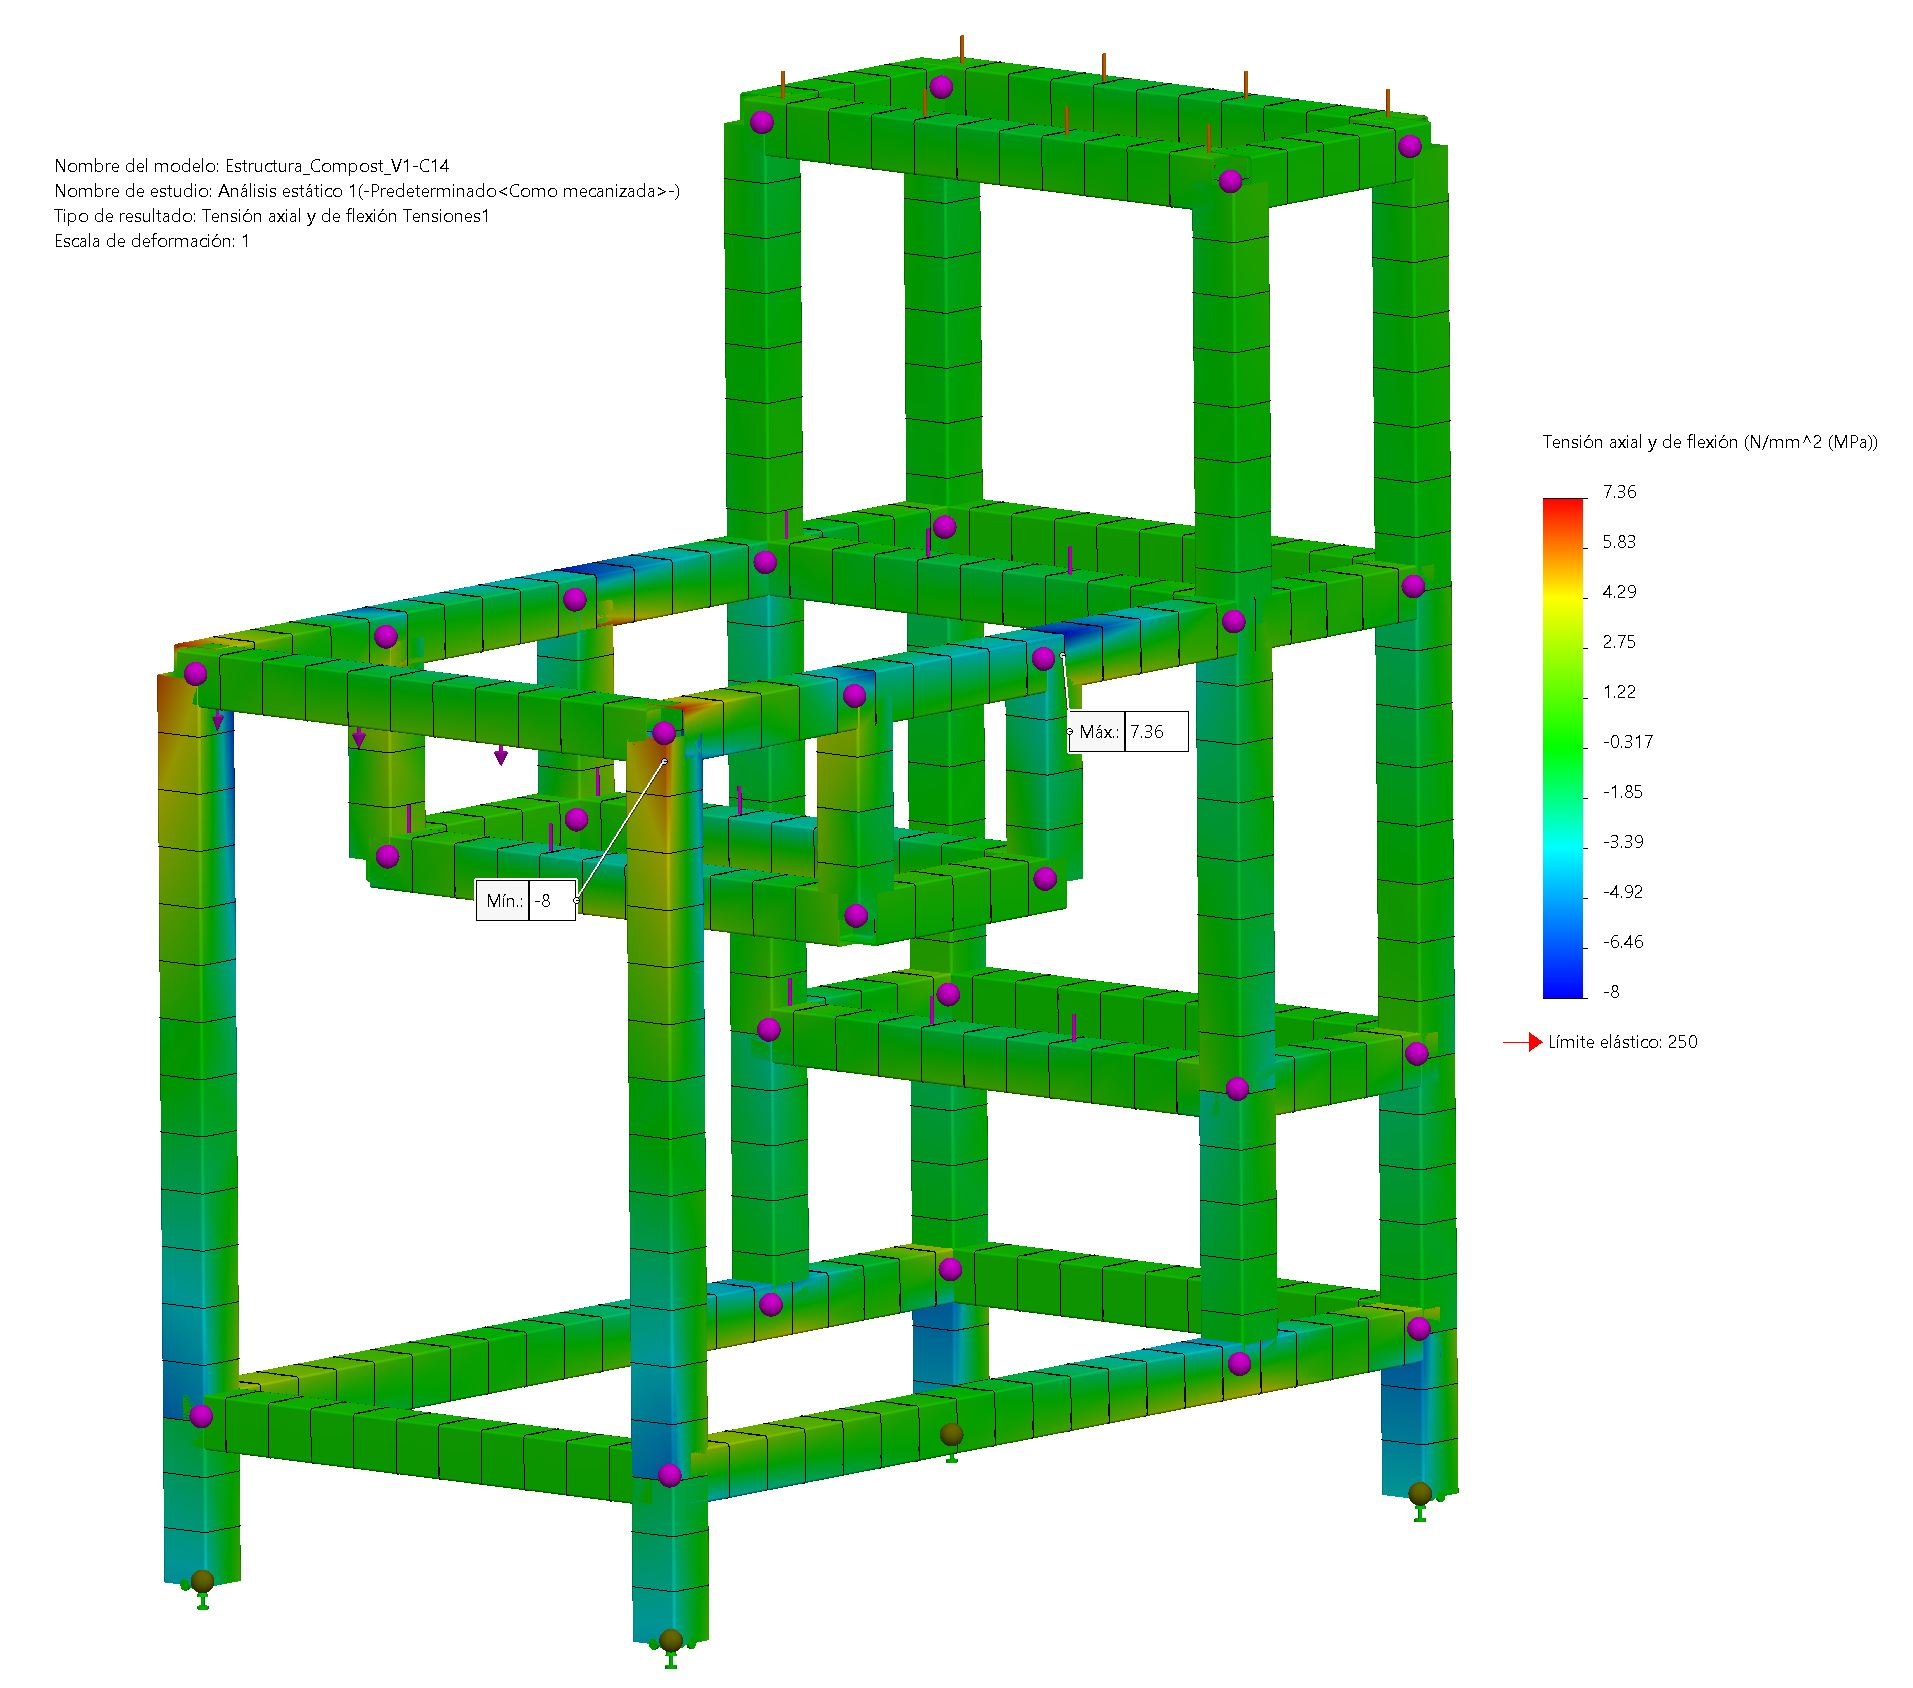
\includegraphics[scale=0.25]{images/Capitulo 4/S6/Analisis-Esfuerzos_1.png}
        \caption{Análisis Esfuerzos de la Estructura final}
    \label{fg:Estructura1}
\end{figure}

De la (Figura \ref{fg:Estructura1}) se pueden extraer los valores del Esfuerzo axial y de flexión máximos, así como el limite elástico, para calcular el factor de seguridad de nuestra estructura.

Por lo que el Factor de Seguridad $FS$ es igual a 
 \begin{center}
     $FS = \frac{\tau_{max}}{\tau_{admisible}}=\frac{250}{8.11} = 30.83$\\
 \end{center} 
 \begin{center}     
     $FS \approx 31$
 \end{center} 

En la siguiente imagen, (Figura \ref{fg:FDS}), se observa el factor de seguridad de la estructura, siendo el valor previamente calculado el factor de seguridad más bajo de esta.

 \begin{figure}[h]
    \centering
        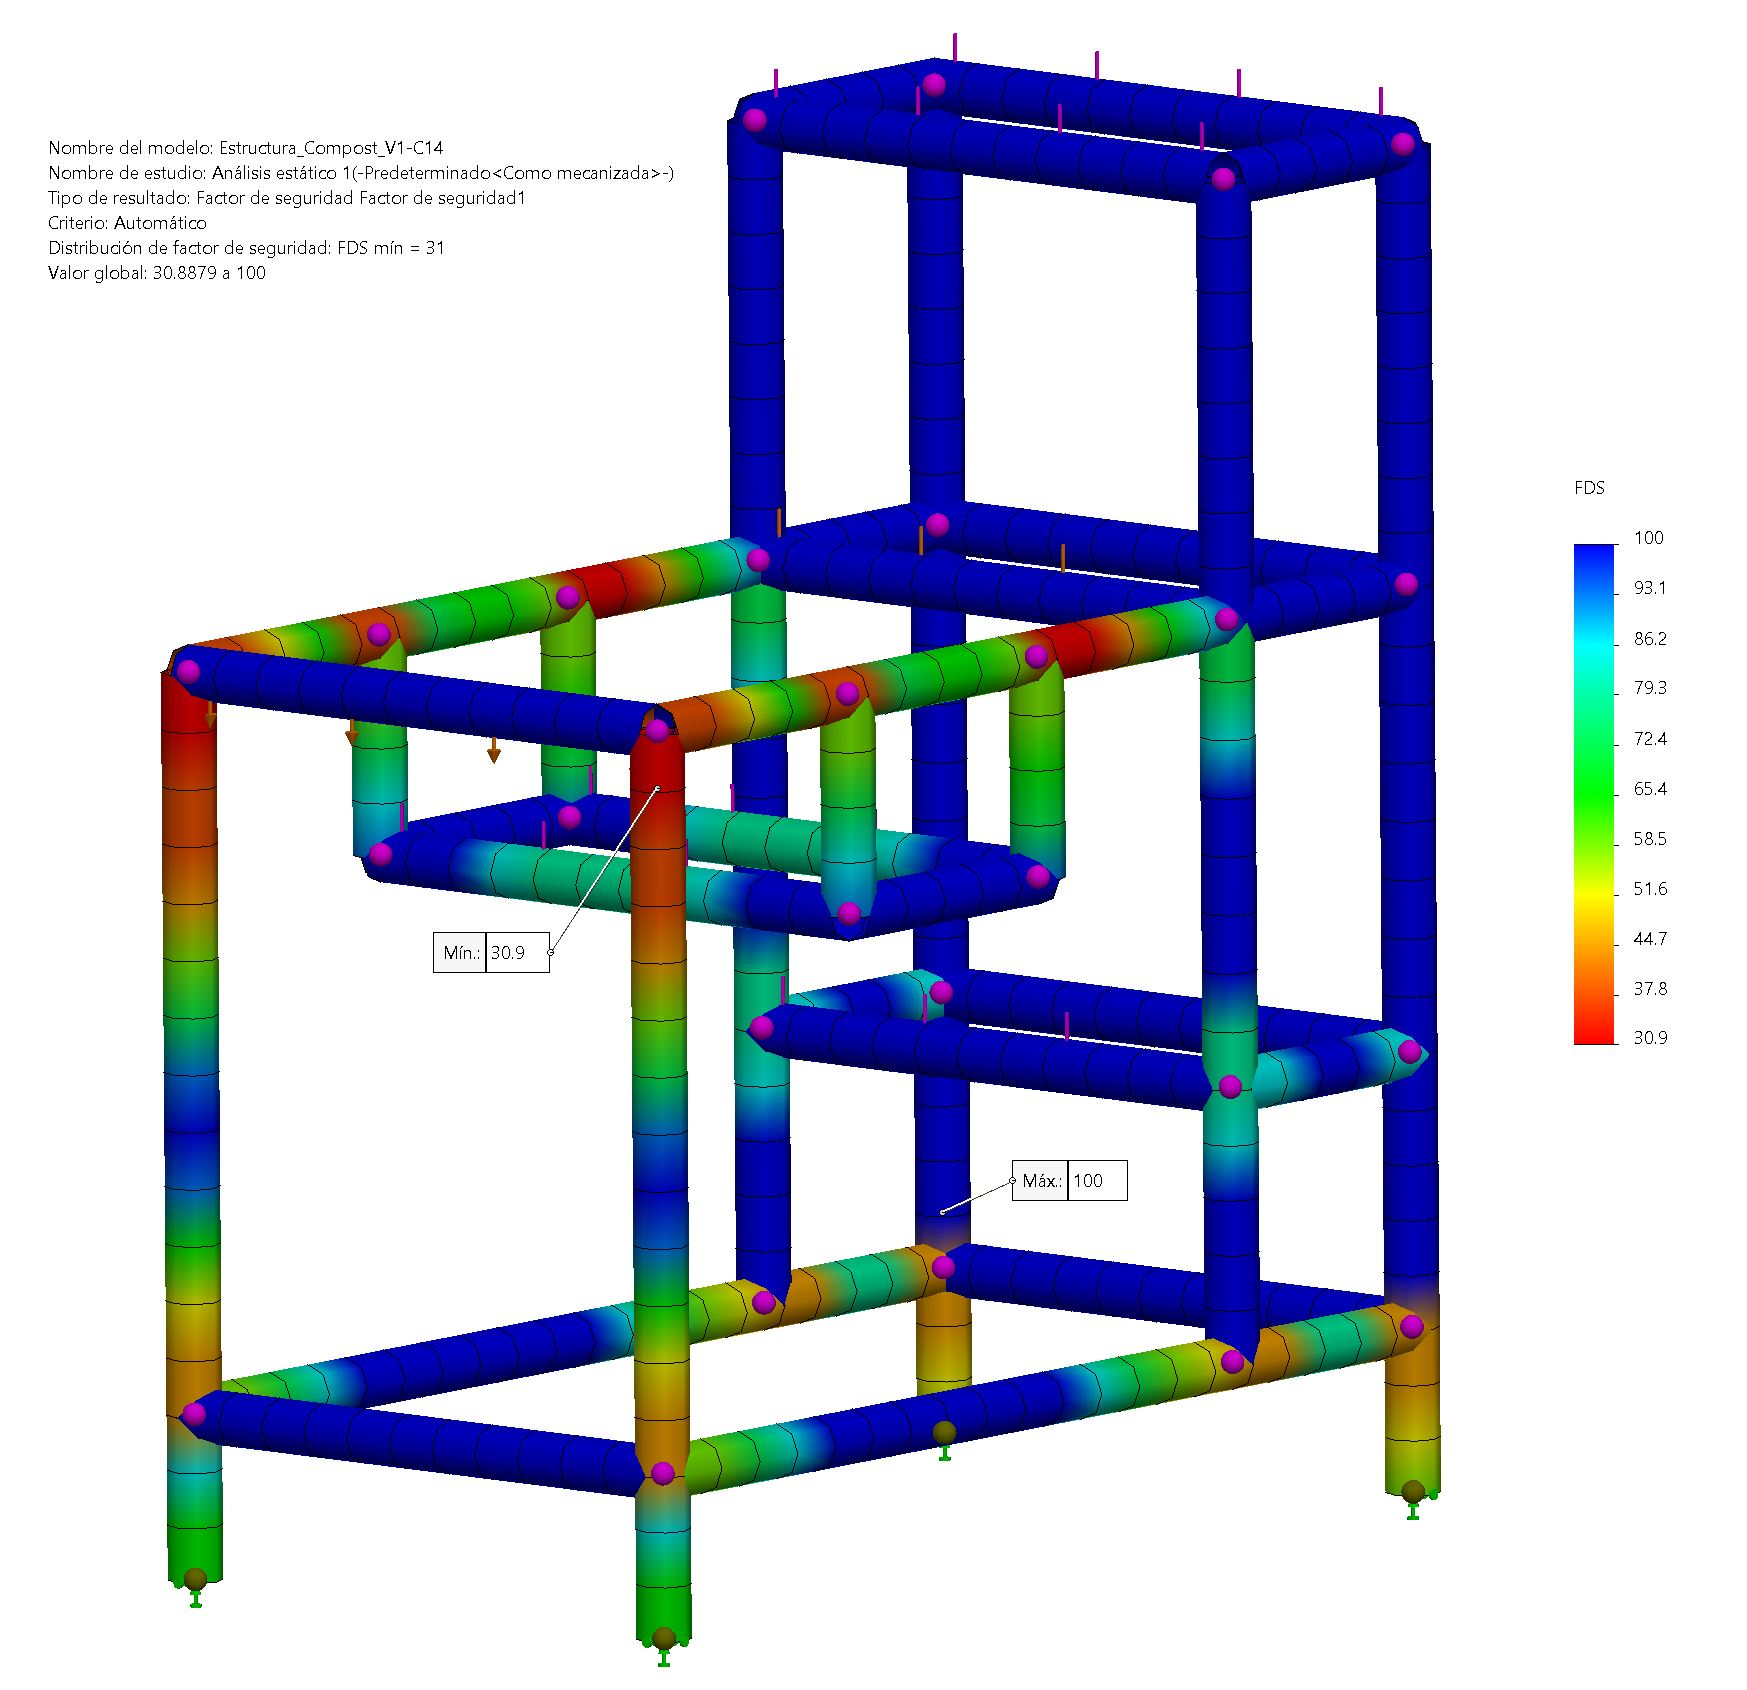
\includegraphics[scale=0.25]{images/Capitulo 4/S6/Analisis-FDS.png}
        \caption{Factor de seguridad en la estructura}
    \label{fg:FDS}
\end{figure}

 En la ultima imagen, (Figura \ref{fg:Estructura2}), también se puede observar que la deformación máxima es de 0.16mm en la parte superior, lo que permite asegurar que el eje no se verá sometido a esfuerzos generados por la deformación de la estructura.

\begin{figure}[h]
    \centering
        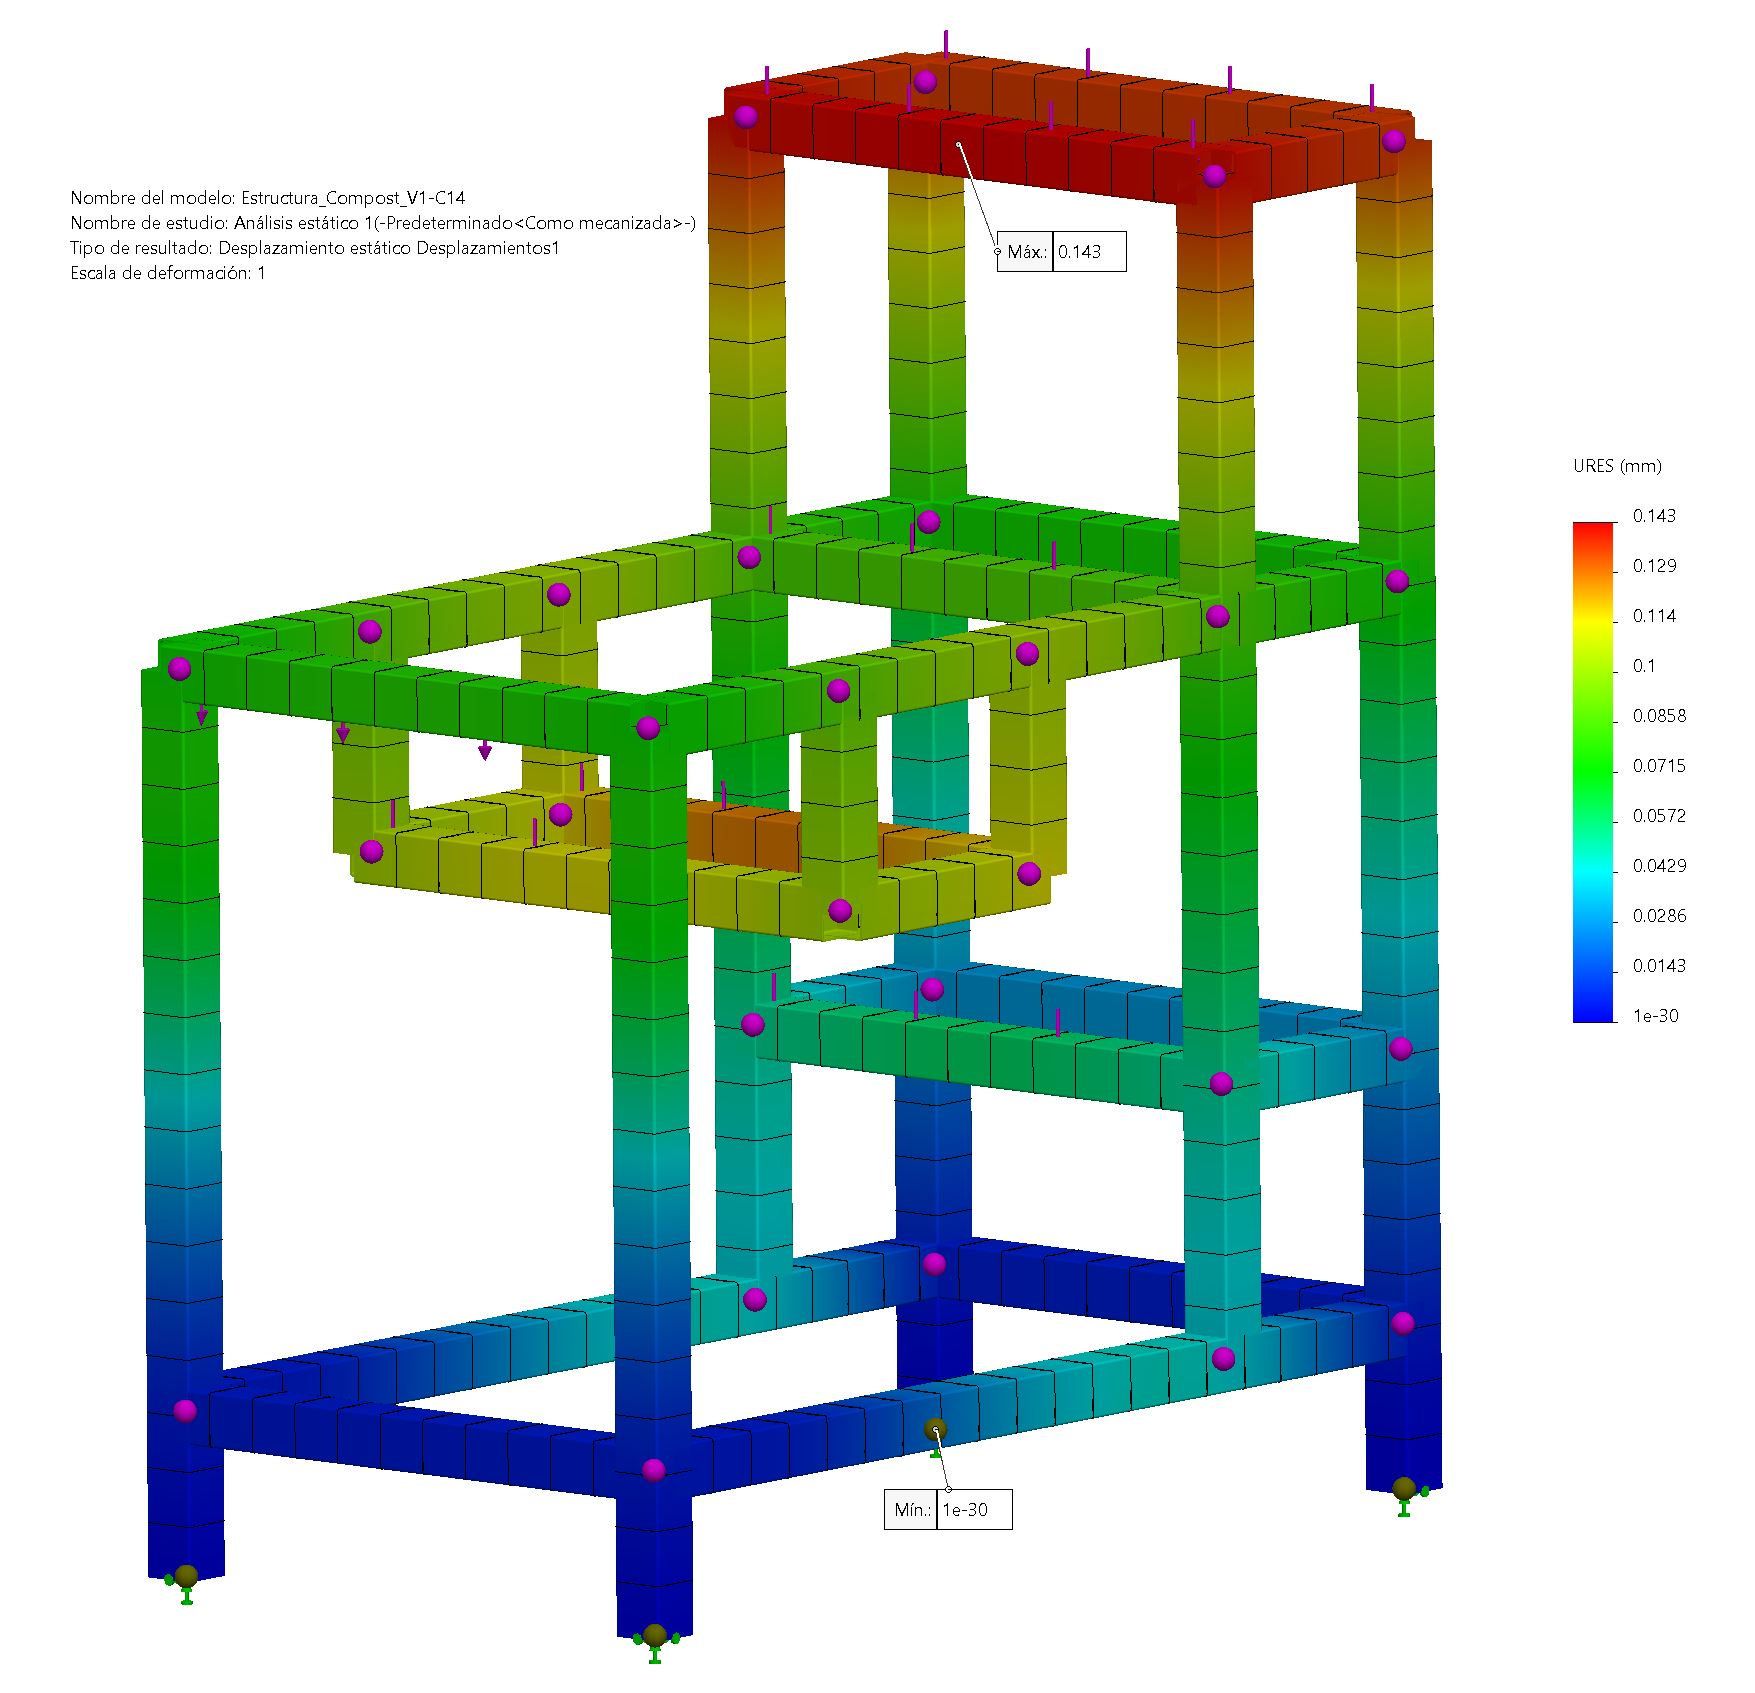
\includegraphics[scale=0.25]{images/Capitulo 4/S6/Analisis-deformacion_1.png}
        \caption{Análisis de Deformación de la Estructura final}
    \label{fg:Estructura2}
\end{figure}


